\documentclass{article}
\usepackage[margin=.5in]{geometry}
\usepackage{graphicx, dblfloatfix}
\usepackage{amsmath, amssymb, amsfonts, mathrsfs, mathtools, physics}
\usepackage[english]{babel}
\usepackage[autostyle, english = american]{csquotes}
\usepackage[normalem]{ulem}
\usepackage[title,titletoc,toc]{appendix}
\usepackage{pgfplotstable}
\usepackage{array, booktabs, colortbl, caption}
\MakeOuterQuote{"}

\newcommand{\redchi}{$\tilde{\chi}^2\,$}
\renewcommand{\vec}[1]{\mathbf{#1}}

\title{Relativistic Dispersion Relation for the Free Electron}
\author{Alejandro Legarda}

\begin{document}
\raggedright
\maketitle

\begin{abstract}
We investigate the energy-momentum relation for the free electron over a wide range of energies, using data from gamma photon Compton scattering and the photoelectric effect. We show that a relativistic model is appropriate for the dispersion relation.
\end{abstract}

\tableofcontents
\newpage

\section{Method}

\begin{figure}[!htb]
	\centering
	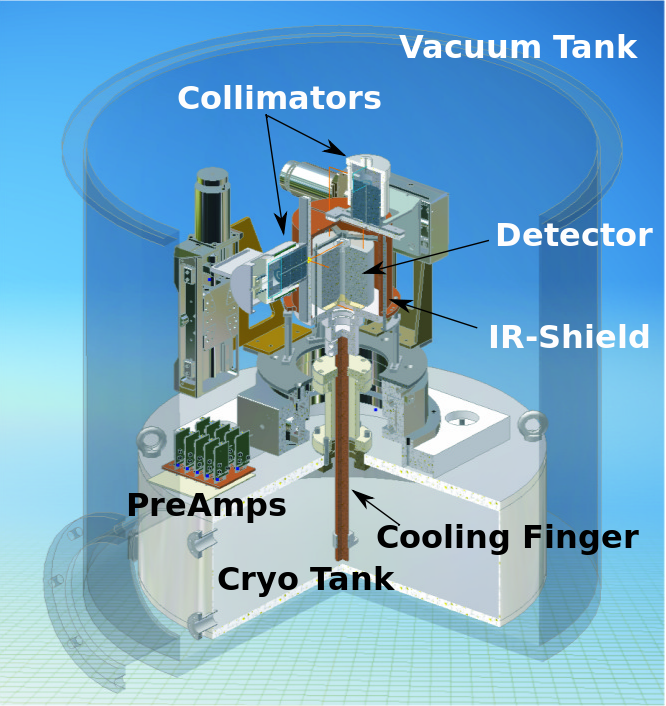
\includegraphics[scale=.5]{plots/galatea_setup_sketch.png}
  	\caption{The Germanium detector. This detector is connected to a pre-amp, which feeds into an amplifier and finally passes the signal on to a PHA, allowing the computer software to produce a histogram based on channel number (energy).} 
 	\label{Apparatus}
\end{figure}

We aim to measure both gamma energies and Compton edges precisely. We use a Germanium detector because of its better energy resolution than sodium-iodide detectors. Gamma radiation from our source enters the Germanium detector and Compton scatters with electrons (or, eventually, undergoes the photoelectric effect), producing electron-hole pairs. This separated charge is collected by the application of a high voltage. The quantity of charge collected is proportional to the energy deposited by the gamma in the crystal. A charge-sensitive pre-amplifier produces pulse heights proportional to the collected charge, an amplifier amplifies the signal, and a pulse height analyzer (PHA) digitizes the pulse heights and displays a histogram of the energies. By measuring features of the resulting spectrum and using momentum and energy conservation, we can independently identify the kinetic energy and momentum of the electrons.

\hspace{0.25cm}

From the PHA's spectrum we are able to extract the energy of the incoming photon, $E_\gamma$, which is represented bu the full energy photopeak. This peak is due to the full energy transfer from the gamma photon to the detector. The process is usually composed of several Compton scatters, but the final interaction is the photoelectric effect, and thus the totality of the photon energy is dumped into the detector.
We also extract the kinetic energy, $T$, given to an electron at a 180 degree scatter. This is observed as the Compton Edge on the spectrum. This is equal to the maximum energy which can be deposited in the detector by a single Compton scatter.

\section{Spectrum Identification and Calibration}

\begin{figure}[!htb]
	\centering
	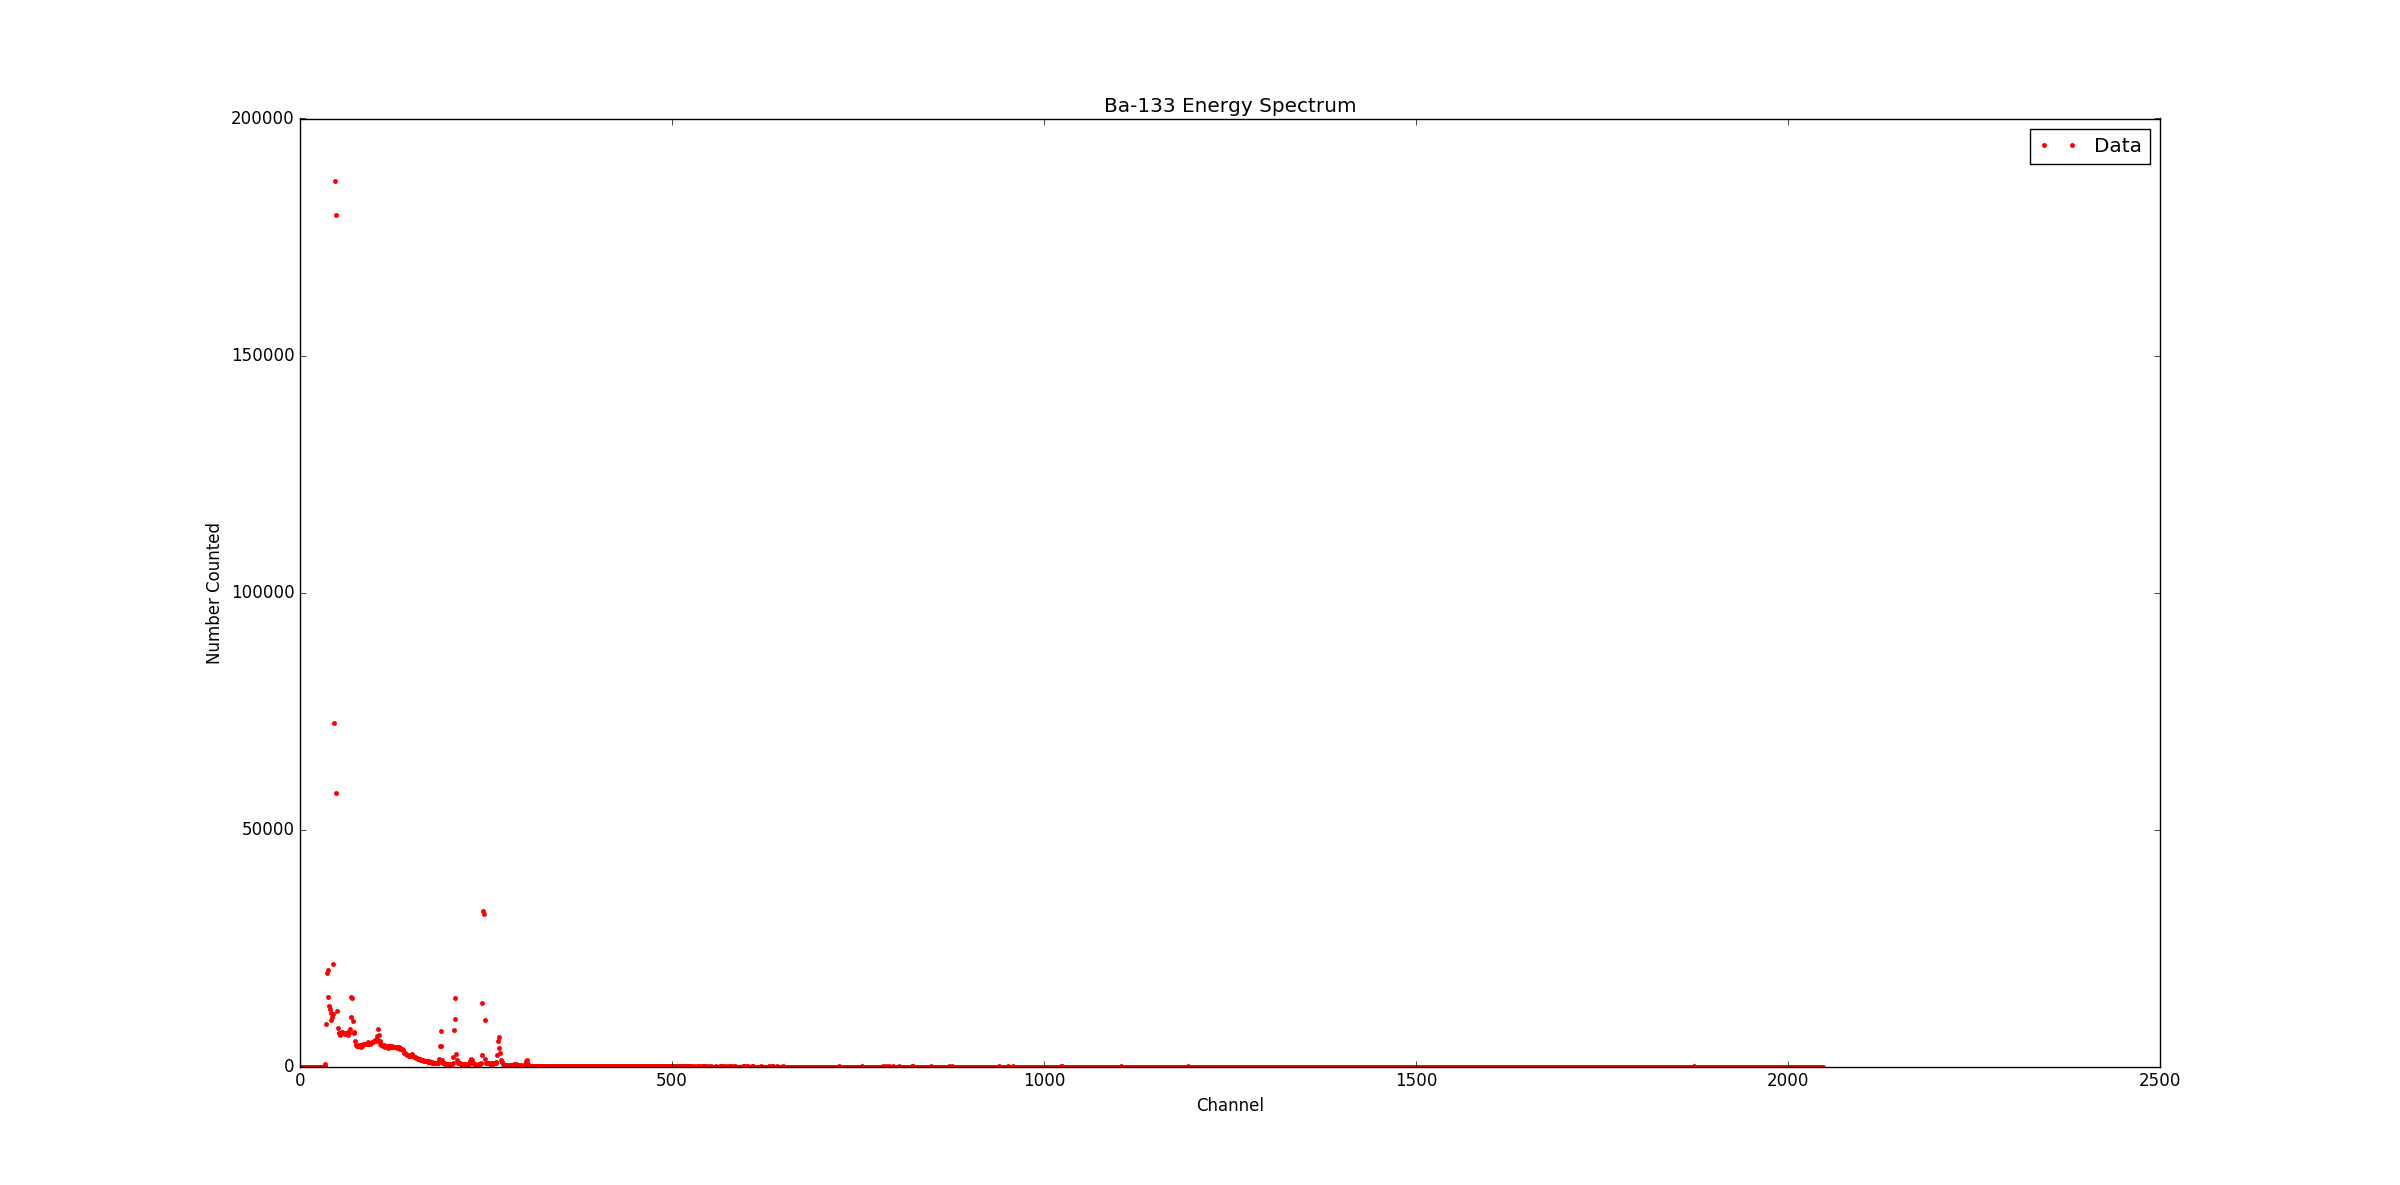
\includegraphics[width = 20cm]{plots/Ba-133_Spectrum.png}
  	\caption{PHA spectrum for Ba-133} 
 	\label{Ba}
\end{figure}

\begin{figure}[!htb]
	\centering
	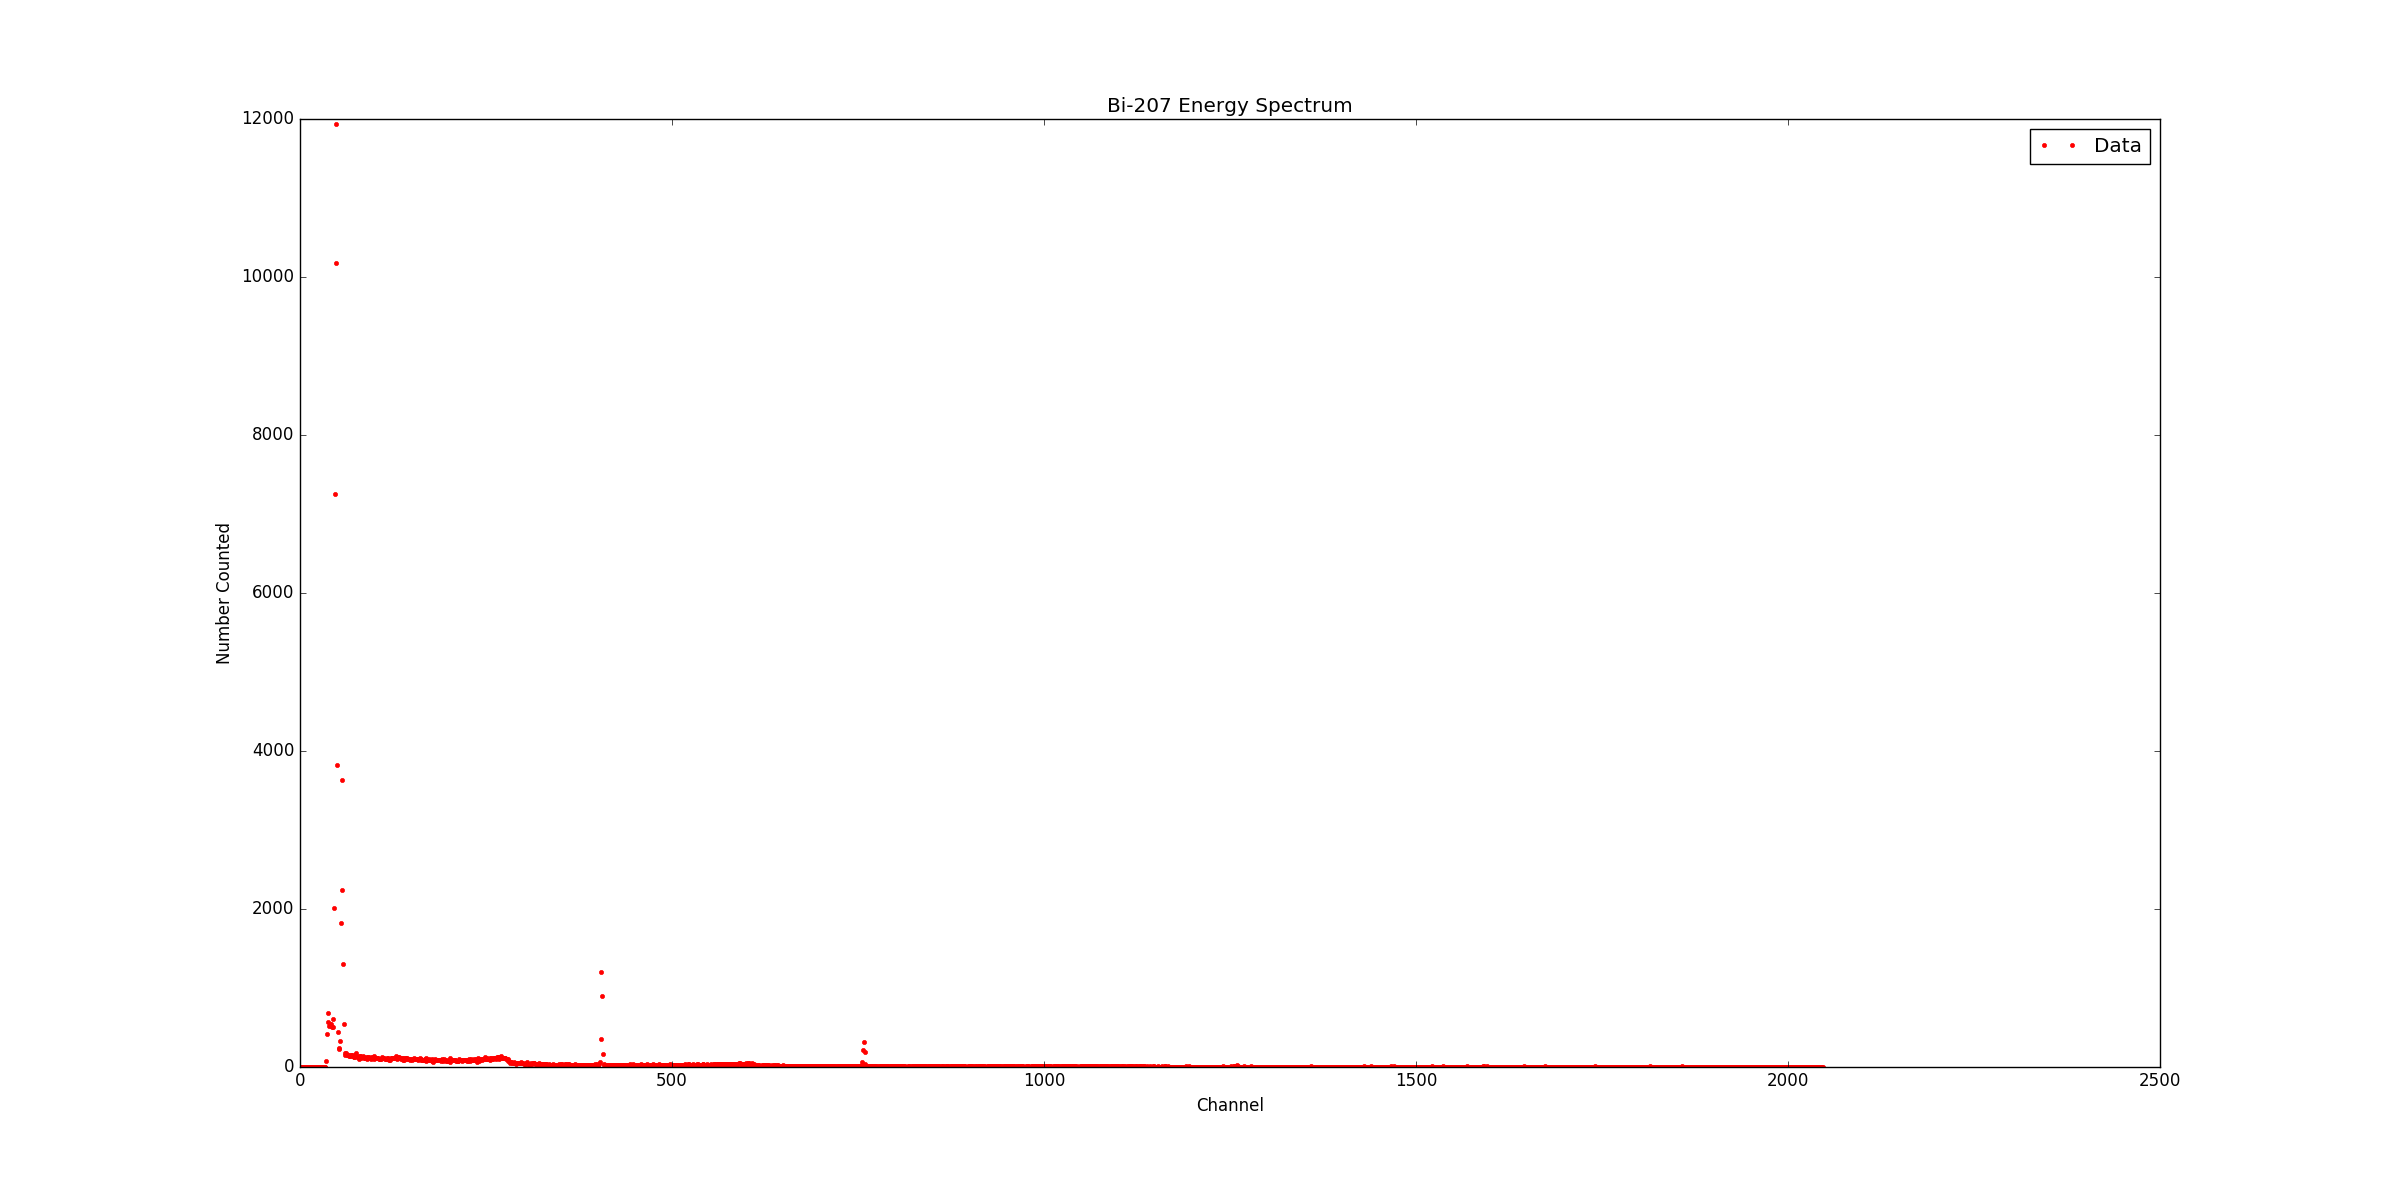
\includegraphics[width = 20cm]{plots/Bi-207_Spectrum.png}
  	\caption{PHA spectrum for Bi-207} 
 	\label{Bi}
\end{figure}

\begin{figure}[!htb]
	\centering
	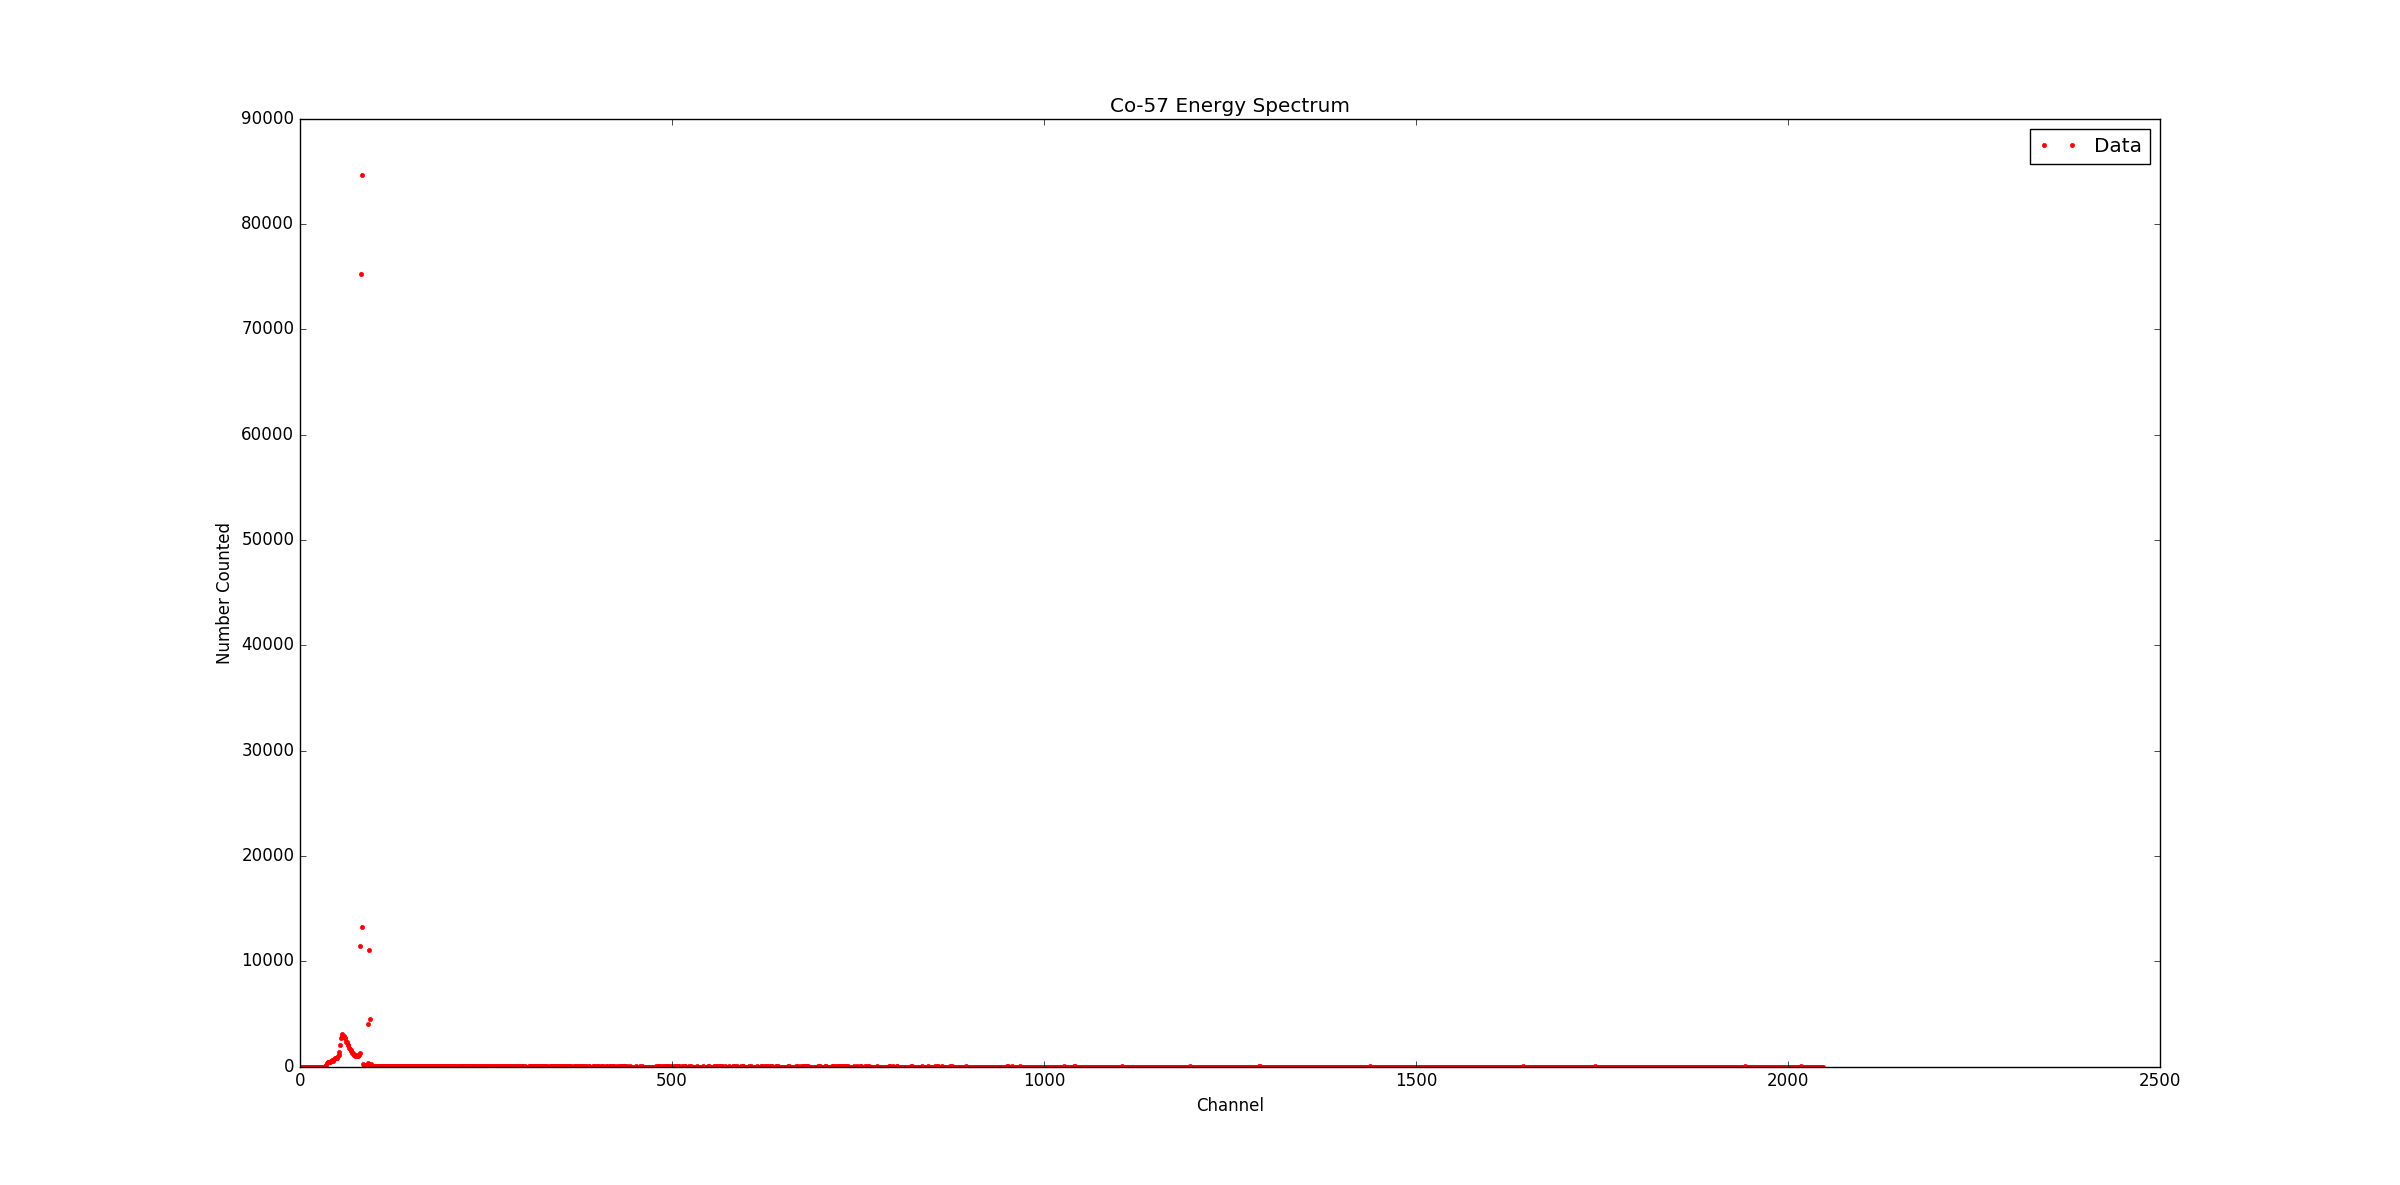
\includegraphics[width = 20cm]{plots/Co-57_Spectrum.png}
  	\caption{PHA spectrum for Co-57} 
 	\label{Co}
\end{figure}

\begin{figure}[!htb]
	\centering
	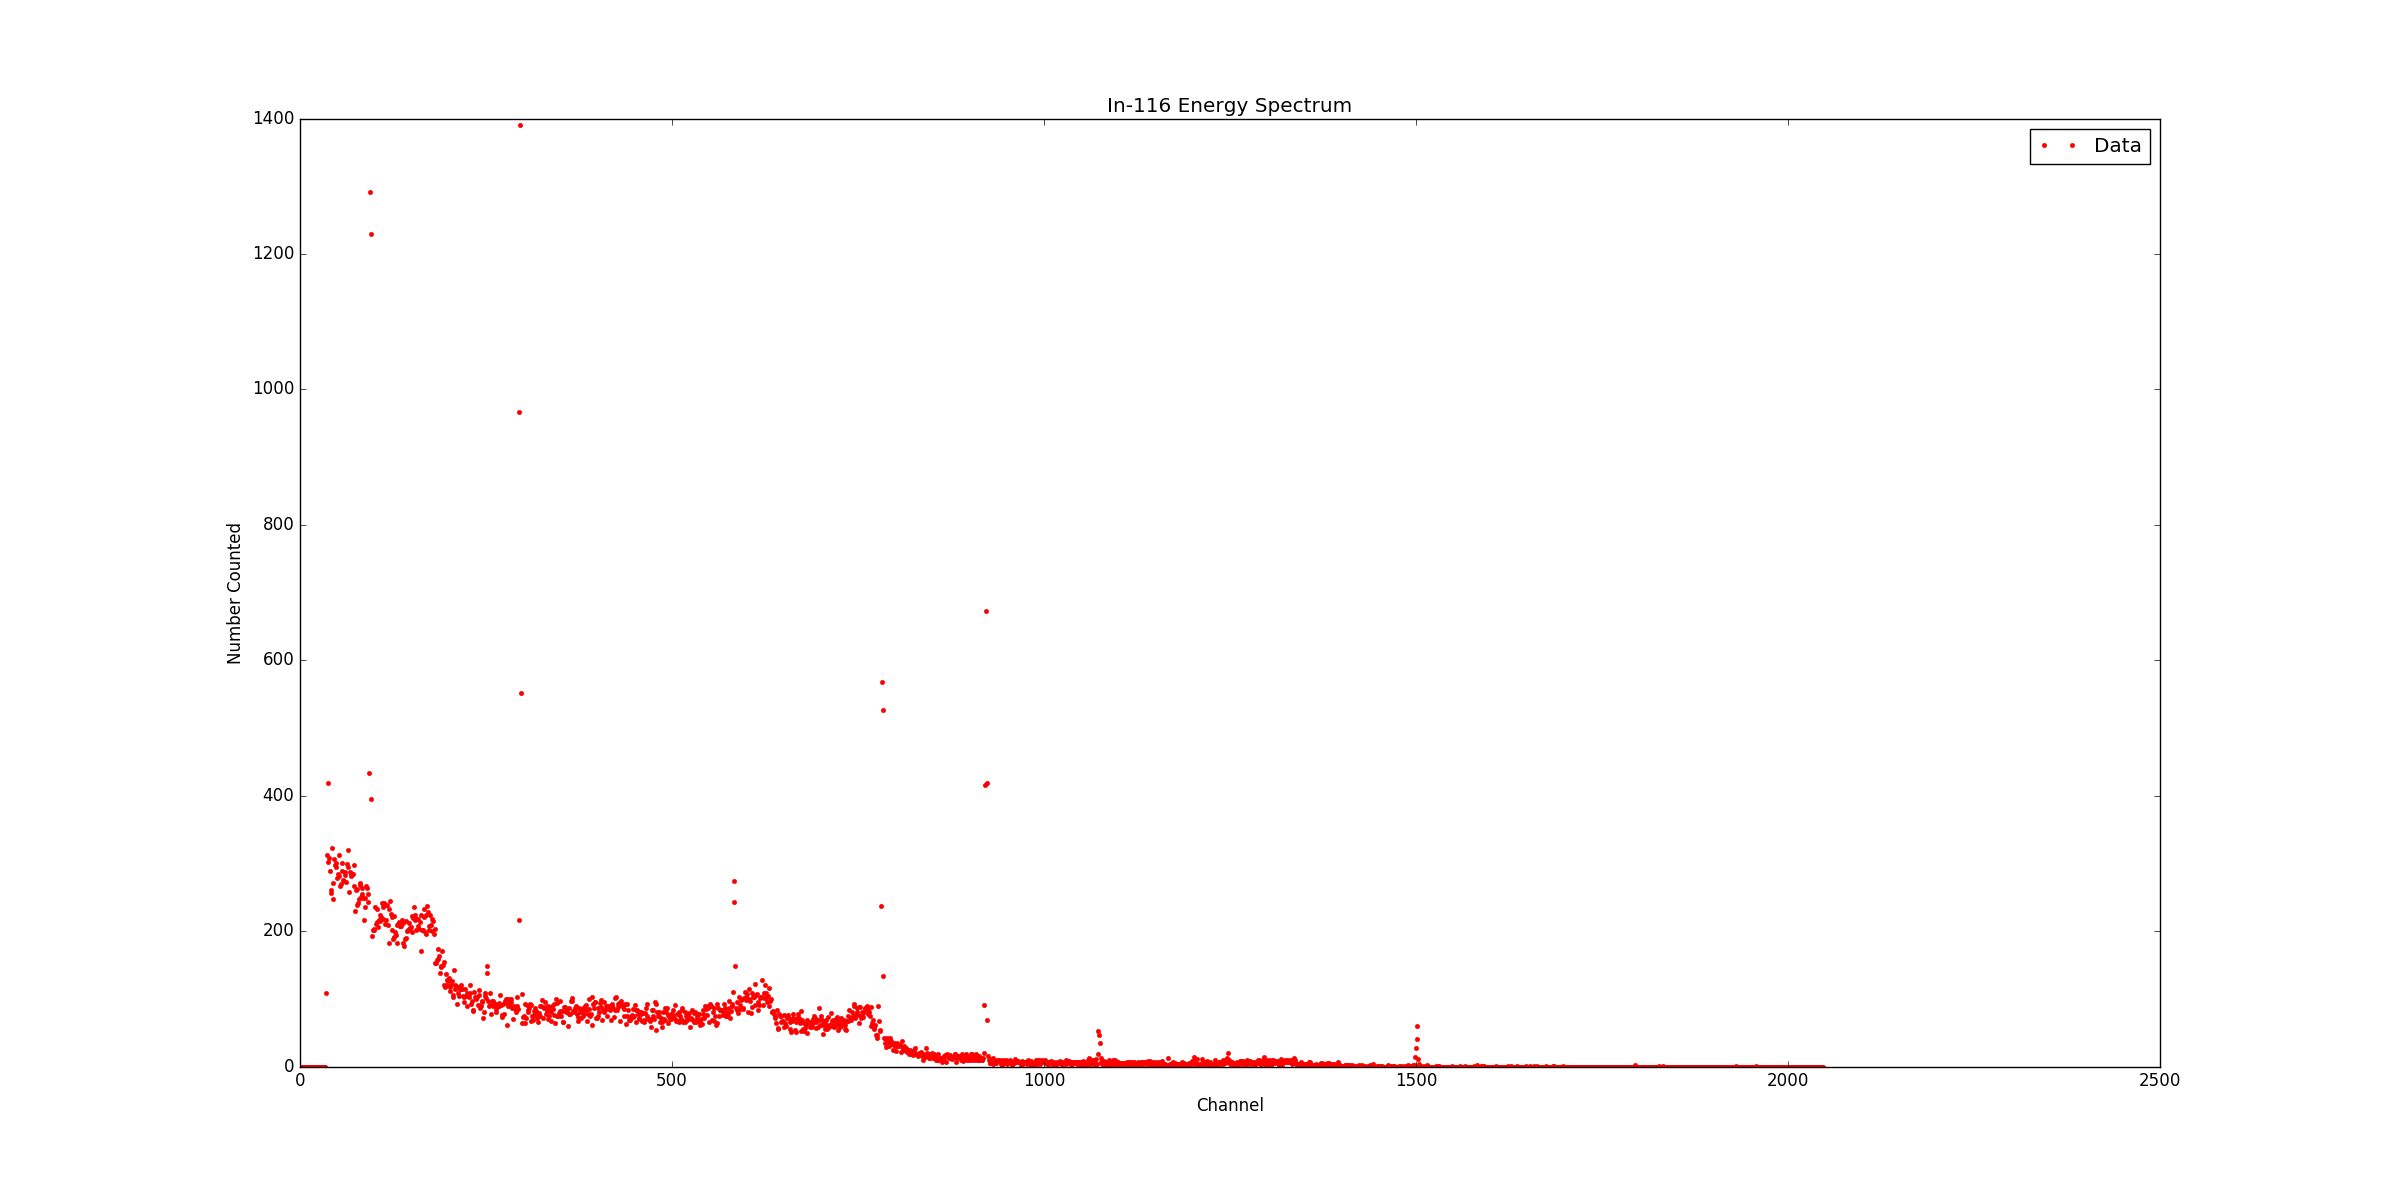
\includegraphics[width = 20cm]{plots/In-116_Spectrum.png}
  	\caption{PHA spectrum for In-116} 
 	\label{In}
\end{figure}

\begin{figure}[!htb]
	\centering
	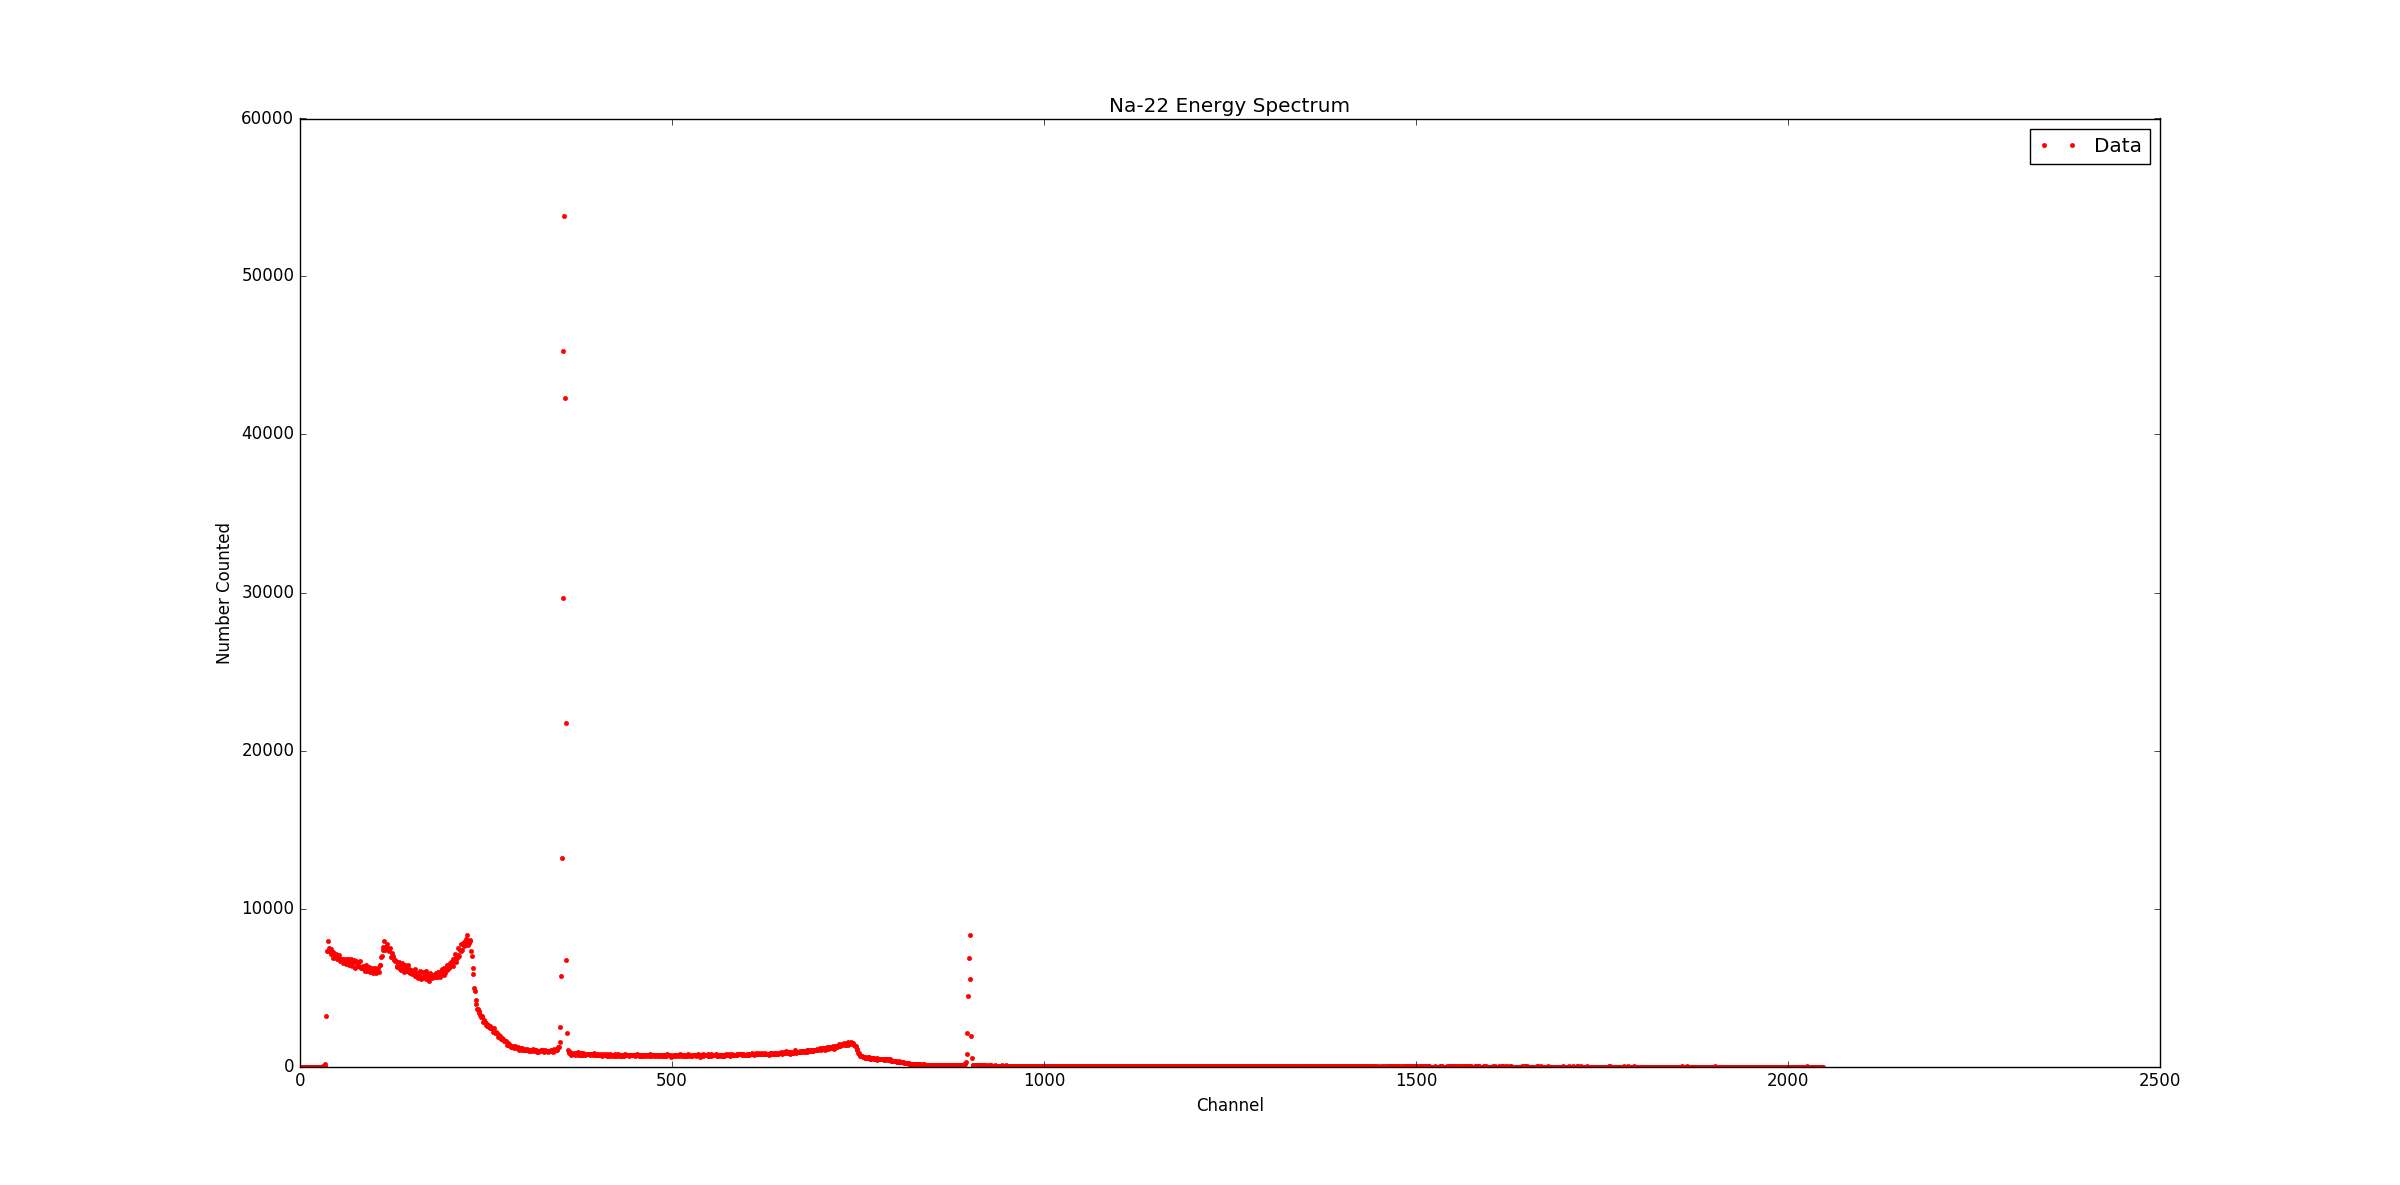
\includegraphics[width = 20cm]{plots/Na-22_Spectrum.png}
  	\caption{PHA spectrum for Na-22} 
 	\label{Na}
\end{figure}

\hspace{.25cm}

Since it is hard to see from the plots due to their scale, we provide a table of Compton edges and full energy peaks. Sources marked with an asterisk (*) indicate that they were used for analysis or calibration (if Compton edge is not present in the row, that indicates it was used for calibration).

\begin{table}[]
\centering
\caption{Compton Edges and Full Energy Peaks}
\label{table}
\begin{tabular}{|c|c|c|c|c|}
\hline
Source & Compton Edge Channel & Uncertainty & Full Energy Peak & Uncertainty \\ \hline
*Cs-137 & 338                  & 3           & 469              & 2           \\ \hline
*Na-22  & 234                  & 3           & 353              & 2           \\ 
*Na-22  & 749                  & 3           & 900              & 2           \\ \hline
Bi-207 &                      &             & 58               & 2           \\ 
*Bi-207 & 279                  & 3           & 405              & 2           \\ 
*Bi-207 & 614                  & 3           & 758              & 2           \\ 
*Bi-207 &                      &             & 1259             & 2           \\ \hline
Co-57  & 65                   & 3           & 83               & 2           \\
Co-57  &                      &             & 93               & 2           \\ \hline
In-116 &                      &             & 94               & 2           \\
*In-116 & 186                  & 4           & 296              & 2           \\ 
In-116 &                      &             & 584              & 2           \\ 
*In-116 & 634                  & 3           & 782              & 2           \\ 
*In-116 & 773                  & 4           & 922              & 2           \\ 
In-116 &                      &             & 1073             & 2           \\ 
In-116 &                      &             & 1501             & 2           \\ \hline
*Ba-133 &                      &             & 46               & 2           \\ 
Ba-133 &                      &             & 69               & 2           \\ 
Ba-133 &                      &             & 105              & 2           \\
Ba-133 &                      &             & 189              & 2           \\ 
Ba-133 &                      &             & 208              & 2           \\
Ba-133 &                      &             & 246              & 2           \\ 
Ba-133 &                      &             & 267              & 2           \\
Ba-133 &                      &             & 289              & 2           \\ 
*Ba-133 &                      &             & 305              & 2           \\ \hline
\end{tabular}
\end{table}

Note how we were unable to discern any Compton Edges from Ba-133's PHA spectrum - this was due to the complexity of Barium's nuclear decay scheme, which makes it hard to discern the locations of peaks let alone Compton Edges.

\begin{figure}[!htb]
	\centering
	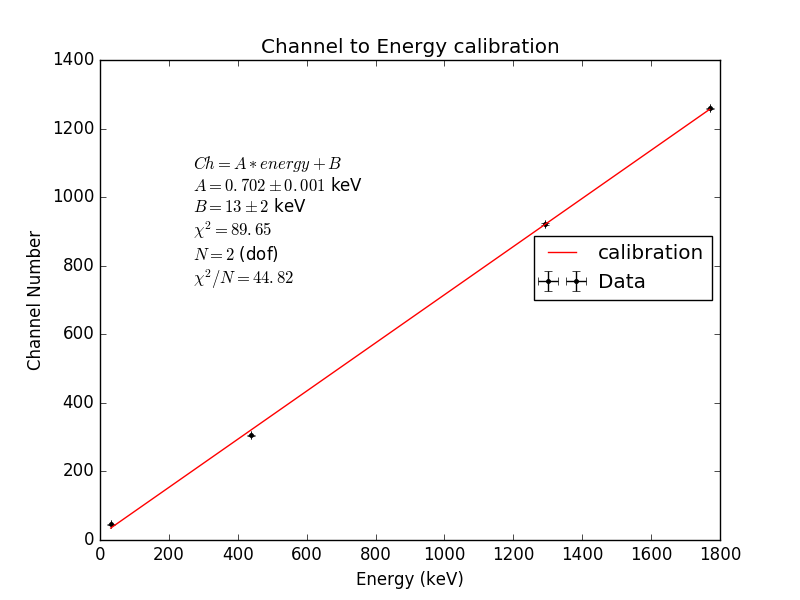
\includegraphics[scale=0.75]{plots/calibration.png}
  	\caption{Channel/Energy Calibration} 
 	\label{calibration}
\end{figure}

\clearpage
\newpage
\section{Analysis}

\begin{figure}[!htb]
	\centering
	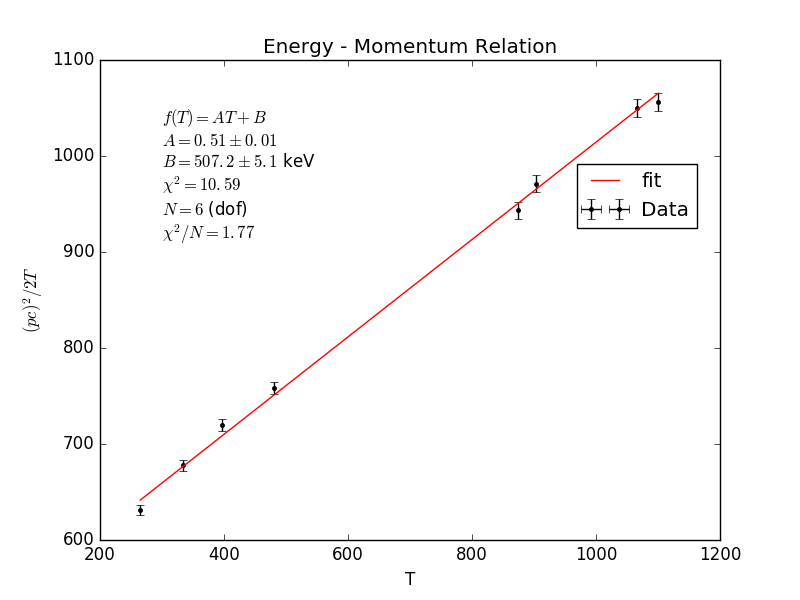
\includegraphics[scale=0.75]{plots/energy_momentum.png}
  	\caption{Energy/Momentum Relation} 
 	\label{calibration}
\end{figure}

From the energy vs. momentum plot ($(pc)^2/2T$ against $T$), we get a function, $g(T)$ that describes their relation. Note that errors were calculated by propagating from the original measurements of $E_\gamma$ and $T$. From equation (15) in the lab manual, we rearrange to show equivalency:

\begin{gather}
	(p c)^2 = 2 m_0 c^2 T + T^2 \\
	\frac{(p c)^2}{2T} = m_0 c^2 + \frac{T^2}{2} \\
\end{gather}

From the fit we have the relation $g(T) ~ \frac{T}{2}$ to satisfaction. Our fit then gives us an electron rest mass value of $m_0 c^2 = 507 \pm 5 keV$, which agrees well with the literature value of $511 keV$. We see that at low T ($T<<2m_0 c^2$), the constant term dominates and therefore we recover the classical equation

\begin{gather}
	(p c)^2 = 2 m_0 c^2 T \\
	\frac{p^2}{2T} = m_0.  \\
\end{gather}

\begin{figure}[!htb]
	\centering
	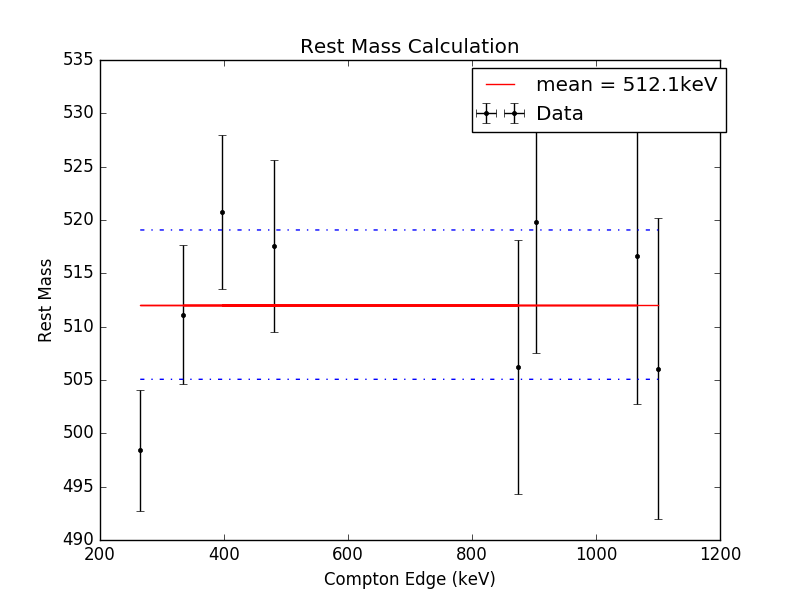
\includegraphics[scale=0.75]{plots/restmass_T.png}
  	\caption{Electron Rest Mass} 
 	\label{calibration}
\end{figure}

From direct rest mass calculation we obtain an average of $m_0 c^2 = 512 \pm 7 keV$, where in this case the error was calculated using a simple standard deviation form the mean. This agrees well with the literature value of $511 keV$.

\begin{figure}[!htb]
	\centering
	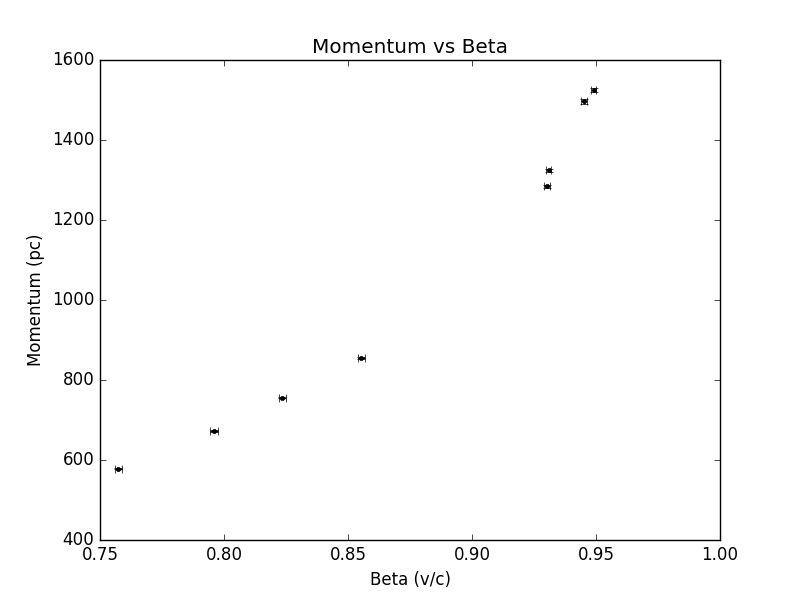
\includegraphics[scale=0.75]{plots/momentum_beta.png}
  	\caption{Electron Rest Mass} 
 	\label{calibration}
\end{figure}

\begin{figure}[!htb]
	\centering
	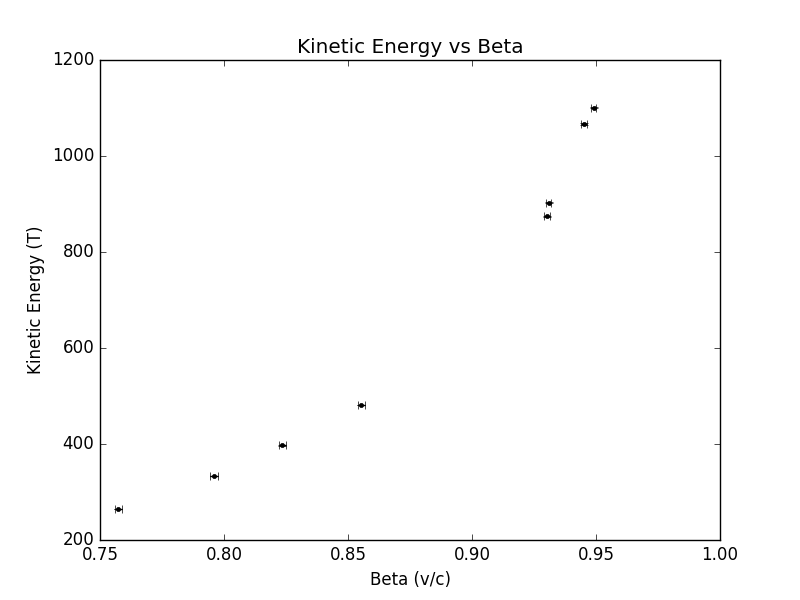
\includegraphics[scale=0.75]{plots/T_beta.png}
  	\caption{Electron Rest Mass} 
 	\label{calibration}
\end{figure}

\hspace{.25cm}
Plotting either momentum or energy against $\beta$ ($v/c$), we can see that as $\beta \rightarrow 1$, both momentum and energy diverge exponentially. This is because no system with mass can achieve $\beta = 1$, i.e., an infinite quantity of energy/momentum would be required to do so. Insight about the form of these plots can be acquired by examining the real mass energy, equation, which includes $\gamma = \frac{1}{\sqrt{1 - \beta^2}}$.

\clearpage
\newpage
\section{Discussion}

It is clear that if we wish to have a relationship that tolerates any value of $T$, we must use the special relativistic model of the dispersion relation. A classical model would have produced a terrible fit since it is evident from our plot that $\frac{(pc)^2}{2T^2}$ does not equal a constant. For high-energy particle physics it is essential that relativity be taken into account.

We found that our calculated electron rest masses agree well with the literature values. The largest source of error for these was the uncertainty in the channel number for the Compton Edges, since they are hard to pinpoint and interpolation is necessary (to try and figure out the center of the edge).

As explained earlier, as $\beta \rightarrow 1$, momentum and (therefore) energy will diverge to infinity, as $\beta = 1$ is a fundamental spacetime limit only achieved by massless particles.


\begin{thebibliography}{10}

	\bibitem{lab manual}
		University of Chicago Department of Physics. "Relativistic Dispersion Relation for the Free Electron"\\
		https://wiki.uchicago.edu/display/P211manuals/Relativistic+Dispersion+Relation+for+the+Free+Electron. (Accessed March, 2016)

	\bibitem{taylor}
		Taylor, John. \emph{An Introduction to Error Analysis}. Sausalito: University Science Books, 1997.
		
\end{thebibliography}


\end{document}